\section{Cronograma de Trabajo}

Para garantizar el cumplimiento riguroso de los hitos del CCCD 2026, el equipo PDA STARS estructuró un plan de trabajo dividido en fases secuenciales: diseño preliminar, simulación aerodinámica, manufactura aditiva y mecánica, integración de aviónica, pruebas en tierra (estabilidad, eyección y banco de sensores), revisión crítica (CDR) y preparación para la campaña de lanzamiento.

\begin{figure}[H]
\centering
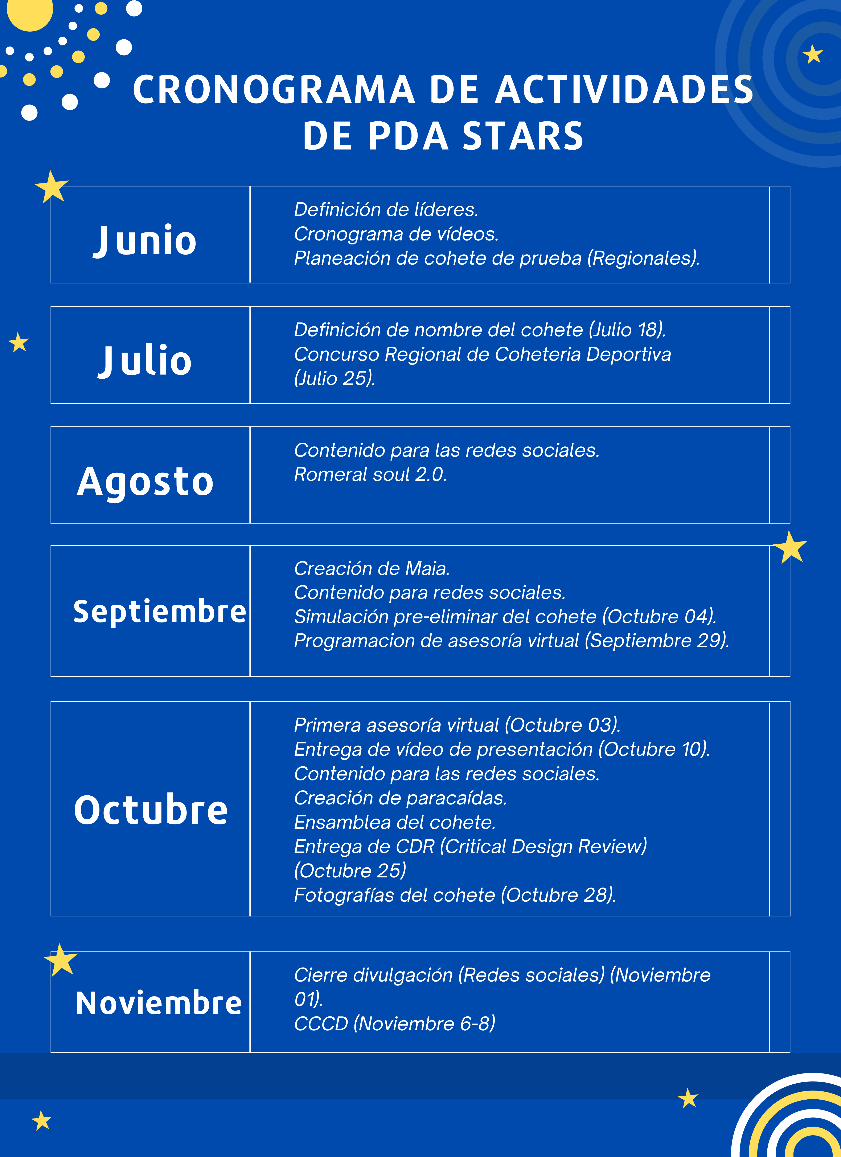
\includegraphics[width=0.95\linewidth]{cronograma_gantt.png}
\caption{Diagrama de Gantt y cronograma general de actividades del proyecto PDA STARS.}
\label{fig:cronograma_actividades}
\end{figure}

El cronograma evidencia la culminación exitosa de las fases de diseño y manufactura estructural, habiendo validado el margen de estabilidad en tierra y la respuesta de la carga útil experimental antes de la fecha límite de entrega de este reporte CDR.
